% CAST MANUAL LATEX
% This is the official manual for the CAST program package
\documentclass[10pt,a4paper]{article} %DOCUMENTCLASS

%%%% PACKAGES
\usepackage[utf8]{inputenc} %ENCODING
\usepackage[english]{babel} %ENGLISH LANGUAGE STYLE
\usepackage[parfill]{parskip} %PARAGRAPH SPACING
\usepackage{color} %COLOURS
\usepackage{tabularx} %BETTER TABLES THROUGH tabularx
\usepackage{listings} %ENABLE (SOURCE) CODE LISTINGS
\usepackage{underscore} %AUTOMATICLY ESCAPING UNDERSCORES
\usepackage{graphicx} %LATEX CANT MANAGE IMAGES, SO WE NEED THIS
\usepackage{hyperref} %ENABLE URL SUPPORT
\usepackage[backend=bibtex,style=chem-angew,biblabel=dot]{biblatex} %REFERENCES
\addbibresource{castManualReferences.bib} %ADD BIBLATEX REFERENCES FILE.
\usepackage{acronym} %SUPPORT FOR ABBREVIATIONS


%%%%OPTIONS FOR CODE LISTINGS
\lstset{ %
	backgroundcolor=\color{white},   % choose the background color; you must add \usepackage{color} or \usepackage{xcolor}
	basicstyle=\footnotesize,        % the size of the fonts that are used for the code
	breakatwhitespace=false,         % sets if automatic breaks should only happen at whitespace
	breaklines=true,                 % sets automatic line breaking
	%captionpos=b,                    % sets the caption-position to bottom
	frame=single,	                 % adds a frame around the code
	keepspaces=true,                 % keeps spaces in text, useful for keeping indentation of code (possibly needs columns=flexible)
	%language=Octave,                 % the language of the code
	numbers=left,                    % where to put the line-numbers; possible values are (none, left, right)
	numbersep=5pt,                   % how far the line-numbers are from the code 
	showspaces=false,                % show spaces everywhere adding particular underscores; it overrides 'showstringspaces'
	showstringspaces=false,          % underline spaces within strings only
	showtabs=false,                  % show tabs within strings adding particular underscores
	stepnumber=1,                    % the step between two line-numbers. If it's 1, each line will be numbered
	tabsize=2,	                     % sets default tabsize to 2 spaces
}

%%%%AUTHOR INFORMATION
\title{CAST Manual}
\author{Working Group Engels \\
	Julius-Maximilians Univeristy Wuerzburg \\
	Wuerzburg, Germany}

%%%%%%%%%%%%%%%%%%%%%%%%%%%%%%%%%%%%
%%%%                            %%%%
%%%%     CONDITIONALS           %%%%
%%%%                            %%%%
%%%%%%%%%%%%%%%%%%%%%%%%%%%%%%%%%%%%
% Different versions of the manual generatable through custom conditionals
\newif\ifverbose %VERBOSE
%VERBOSE: Use this conditional to describe procedures in detail or write detailed usage describtions which bloat the manual.

\newif\ifdevelopment %DEVELOPMENT
%DEVELOPMENT: Notes for people who have access to the CAST source and / or are coding inside CAST

\newif\ifdevmode %DEVMODE
%DEVMODE: Notes we (the authors of this manual) pass to each other.

\devmodetrue
\verbosetrue
\developmenttrue

\begin{document}
	\pagenumbering{Roman}
	%%%%%%%%%%%%%%%%%%%%%%%%%%%%%%%%%%%%
	%%%%                            %%%%
	%%%%     TITLE PAGE             %%%%
	%%%%                            %%%%
	%%%%%%%%%%%%%%%%%%%%%%%%%%%%%%%%%%%%

	% FRONT PAGE

	CAST - Conformational Search and Analysis Tool

	\ifdevelopment
		Manual for developers and programmers
	\else
		Manual
	\fi

	\ifverbose\else
		quick reference - short version
	\fi

	\ifdevmode
		\colorbox{red}{DEV MODE! THIS MANUAL IS NOT DESTINED TO BE RELEASED!}
	\fi

	Version 3.1 \\
	\today

	\ifdevmode
	\colorbox{red}{WE SHOULD REALLY PUT THE CAST ICON HERE!}
	\fi


	%%%%%%%%%%%%%%%%%%%%%%%%%%%%%%%%%%%%
	%%%%                            %%%%
	%%%%     TABLE OF CONTENTS      %%%%
	%%%%                            %%%%
	%%%%%%%%%%%%%%%%%%%%%%%%%%%%%%%%%%%%
	\newpage
	\tableofcontents

	%%%%%%%%%%%%%%%%%%%%%%%%%%%%%%%%%%%%
	%%%%                            %%%%
	%%%%     LIST OF FIGURES        %%%%
	%%%%                            %%%%
	%%%%%%%%%%%%%%%%%%%%%%%%%%%%%%%%%%%%

	\newpage
	\listoffigures

	%%%%%%%%%%%%%%%%%%%%%%%%%%%%%%%%%%%%
	%%%%                            %%%%
	%%%%     LIST OF TABLES         %%%%
	%%%%                            %%%%
	%%%%%%%%%%%%%%%%%%%%%%%%%%%%%%%%%%%%
	\newpage
	% We don't need this right now
	%\listoftables

	%%%%%%%%%%%%%%%%%%%%%%%%%%%%%%%%%%%%
	%%%%                            %%%%
	%%%%     LIST OF ABBREVIATIONS  %%%%
	%%%%                            %%%%
	%%%%%%%%%%%%%%%%%%%%%%%%%%%%%%%%%%%%
	\section{Table of Abbreviations}
	\begin{acronym}[DEINEMUDDA] % längste Abkürzung steht in eckigen Klammern
		\setlength{\itemsep}{-\parsep} % geringerer Zeilenabstand
		\acro{AMBER}{Assisted Model Building with Energy Refinement}
		\acro{AMOEBA}{Atomic Multipole Optimized Energetics for Biomolecular Applications}
		\acro{CAST}{Conformational Analysis and Search Tool}
		\acro{CHARMM}{Chemistry at Harvard Macromolecular Mechanics}
		\acro{DFT}{Density Functional Theory}
		\acro{DFTB}{Density Functional Tight Binding}
		\acro{DOF}{degree of freedom}
		\acrodefplural{DOF}[DOFs]{degrees of freedom}
		\acro{dRMSD}{distance root-mean-square deviation}
		\acro{FEP}{Free Energy Pertubation}
		\acro{GAFF}{General Amber Force Field}
		\acro{GCC}{GNU Compiler Collection}
		\acro{GPU}{graphics processing unit}
		\acro{MC}{Monte-Carlo}
		\acro{MCM}{Monte-Carlo with Minimization}
		\acro{MD}{Molecular Dynamics}
		\acro{MOPAC}{Molecular Orbital Package}
		\acro{MPI}{Message Parsing Interface}
		\acro{NEB}{Nudged Elastic Band}
		\acro{NMR}{nuclear magnetic resonance}
		\acro{OPLS-AA}{Optimized Potentials for Liquid Simulations All-Atoms}
		\acro{PBC}{Periodic Boundary Conditions}
		\acro{PCA}{Principal Component Analysis}
		\acro{PDF}{probability density function}
		\acro{PES}{potential energy surface}
		\acro{PME}{Particle Mesh Ewald}
		\acro{RMSD}{root-mean-square deviation}
		\acro{SAPT-FF}{Symmetry Adapted Perturbation Theory based Force Field}
		\acro{SPME}{Smooth Particle Mesh Ewald}
		\acro{TS}{Tabu Search}
		\acro{US}{Umbrella Sampling}
		\acro{VdW}{Van-der-Waals}
		\acro{VMD}{Visual Molecular Dynamics}
		\acro{WHAM}{Weighted Histogram Analysis Method}
	\end{acronym}
	\newpage

	%%%%%%%%%%%%%%%%%%%%%%%%%%%%%%%%%%%%
	%%%%                            %%%%
	%%%%     PREFACE                %%%%
	%%%%                            %%%%
	%%%%%%%%%%%%%%%%%%%%%%%%%%%%%%%%%%%%
	\pagenumbering{arabic}
	\section{Preface}
	The \ac{CAST} allows the accurate treatment of large and flexible (macro-)molecular systems. For the determination of thermally accessible minima \ac{CAST} offers the newly developed \ac{TS} algorithm\supercite{tabusearch}, as well as \ac{MC}\supercite{mc_original}, \ac{MCM}\supercite{MCM_original} and \acf{MD}\supercite{computer_simulation_of_MD} implementations. For the determination of reaction paths \ac{CAST} provides the PathOpt\supercite{pathopt}, the \ac{NEB}\supercite{neb_original} and the \ac{US}\supercite{umbrella_sampling} approach. Access to free energies is possible through the \ac{FEP} approach. Along with a number of standard force fields, a newly developed Symmetry Adapted Perturbation Theory based force field (\acs{SAPT-FF}) is included. Semi-Empirical computations are possible through DFTB+\supercite{dftb} (\acl{DFTB}) and \ac{MOPAC}\supercite{mopac, mopac_parallel} interfaces. For calculations based on \ac{DFT}, a \ac{MPI} to the \acs{GPU} accelerated TeraChem\supercite{terachem} program is available. For more information on \ac{CAST} see \cite{cast}.
	\newpage


	%%%%%%%%%%%%%%%%%%%%%%%%%%%%%%%%%%%%
	%%%%                            %%%%
	%%%%     COMPILING CAST         %%%%
	%%%%                            %%%%
	%%%%%%%%%%%%%%%%%%%%%%%%%%%%%%%%%%%%
	\ifdevelopment
	\section{Compiling CAST}
	The \ac{CAST} source code is not openly distributed. Currently, \ac{CAST} in principle has no external dependencies. The \ac{PME} code however at this point still depends on FFTW libraries and is therefore not enabled by default. If you need to perform simulations with \ac{PME}, please contact the \ac{CAST} developers. Compilation was verified using Microsoft Visual Studio 2015 Update 1 on Windows 10 and \acs{GCC} 5.3 on SuseLinux. A makefile for Linux operating systems is part of the source code repository.
	
	The source code is currently kept on a private GitHub repository. If you feel that you are entitled to access to the repository, please contact the \ac{CAST} developers and get an invitation.
	\fi
	\newpage
	%%%%%%%%%%%%%%%%%%%%%%%%%%%%%%%%%%%%
	%%%%                            %%%%
	%%%%       Installation         %%%%
	%%%%                            %%%%
	%%%%%%%%%%%%%%%%%%%%%%%%%%%%%%%%%%%%

	\section{Installation}
	\ac{CAST} is usually distributed as a precompiled executable for Linux and Windows. Currently \ac{CAST} has no external dependencies.

	\ifdevelopment
		The Windows binary can be used with any Windows operating system starting from Windows 7. No further requirements exist. On Linux,
		precompiled binaries are statically linked. FFTW 3.4 libraries have to be set in the \textit{PATH} variable of the Linux shell:\\
		\textbf{LD\_LIBRARY\_PATH \glqq Path to FFTW lib dir\grqq}
	\fi
	\newpage

	%%%%%%%%%%%%%%%%%%%%%%%%%%%%%%%%%%%%%%
	%%%%                              %%%%
	%%%% General Structure and Useage %%%%
	%%%%                              %%%%
	%%%%%%%%%%%%%%%%%%%%%%%%%%%%%%%%%%%%%%
	\section{General Structure and Usage}
	\ac{CAST} features several main computation methods which can be combined with force fields, semi-empirical or \ac{DFT} methods via several interfaces. Input file formatting and available commands are discussed in the following paragraphs.


	%%%% Configuration File %%%%
	\subsection{Configuration File}
	A file named \glqq CAST.txt\grqq or \glqq INPUTFILE\grqq~can be used to change the configuration options of \ac{CAST}. It contains option keywords followed by one or more appropriate values. The keywords are case sensitive. Comments can be included by starting the line with a \glqq \#\grqq. The variables are usually of type integer, floating point or boolean (booleans currently being either \glqq 0\grqq~and \glqq 1\grqq~or plain text \glqq true\grqq~and \glqq false\grqq~without quotation marks).\\

	The following input commands are compulsory for \ac{CAST} to work and have to be set for every calculation.\\~\\
	\begin{tabularx}{\textwidth}{l|l|l}
		Variable&	Effect &	Default \\
		\hline
		verbosity &	Amount of \ac{CAST} output &	1\\
		cores &	Number of OpenMP threads &	1\\
		name &	Name of input file &	none\\
		outname &	Name of output files &	none\\
		input-type &	Format of coordinate file &	TINKER\\
	\end{tabularx}\\~\\

	The keyword for the path of the used coordinate file is "name". The variable “cores” controls the number of threads if multi-threated \ac{CAST} is used (i.e. if \ac{CAST} has been compiled with OpenMP\supercite{openmp08}). “outname” defines the name of the outputfile with information regarding the calculation.
	The switch controlling how much information \ac{CAST} will print to the console is named "verbosity". Proper values are positive integral numbers where low numbers indicate less information than higher numbers do. Suggested values for productive use are 1, 2 or 3. In general, lower numbers will yield less obvious output which is  more suitable for processing (since there are less superficial descriptors printed). Higher values may slow down program execution but provide detailed insight into the program's execution. The detailed effect of the numerical verbosity setting depends on the chosen task.

	An example input for a single point energy calculation with \ac{OPLS-AA} Force Field\supercite{oplsaa, oplsaa2} is given below:
	
	\begin{lstlisting}
	verbosity              3
	name                   inputstructure.xyz
	inputtype              TINKER
	outname                thisIsTheOutputFile
	cores                  4
	task                   SP
	interface              OPLSAA
	paramfile              oplsaa.prm\end{lstlisting}

	A more explicit, commented version of the INPUTFILE containing all parameters is distributed with \ac{CAST}.

	%%%% Force Fields %%%%
	\subsection{Force fields}
	\ac{CAST} features four different force field implementations:\\
	\begin{itemize}
	 \item \acf{OPLS-AA}\supercite{oplsaa, oplsaa2} \item \acf{CHARMM}\supercite{charmm}
	 \item \acf{AMBER}\supercite{amber}
	 \item \acf{AMOEBA}\supercite{amoeba_current, amoeba_current2}
	\end{itemize}~\\
	With the exception of the \ac{AMOEBA} force field, the non-bonded parts of the force fields have been parallelized using the OpenMP programming model. Furthermore, the \ac{FEP} and \ac{SPME} methods can only be used with \ac{OPLS-AA}, \ac{CHARMM} and \ac{AMBER}. The force fields have to be in a format similar to the one used by the TINKER\supercite{tinker} program. They may be obtained from the TINKER\supercite{tinker} website.
		%% AMOEBA and short range correction
		\subsubsection{AMOEBA and short range correction}
		\ifdevmode \colorbox{red}{Blalala yaddayaddayadda… insert stuff here.} \fi
		%% Smooth particle Mesh Ewald
		\subsubsection{Smooth particle Mesh Ewald}
		\ac{SPME}\supercite{spme} allows the treatment of full electrostatic in periodic systems. Essential for the use of the \ac{SPME} are applied periodic boundary conditions. \ac{SPME} uses the FFTW 3.4 library for the fourier transformations of the charge grid $($see Installation details$)$.  \ac{SPME} control features the following parameters:\\~\\

		\begin{tabularx}{\textwidth}{l|l|l}
			variable & effect & default \\
			\hline
			PME & Switches pme on or off 0 = off, 1 = on & 0 \\
			PMEspline & Spline order used in SPME & 5 \\
			PMEtreshold & Affects the value of the ewald coefficient & 0.00000001 \\
		\end{tabularx}

		\ifdevmode
		\colorbox{red}{WE NEED TO ADRESS THE FFTW LIB ISSUE!}
		\fi

	%%%% Energy Interfaces %%%%
	\subsection{Energy Interfaces}
	The energy interfaces are the main parts of \ac{CAST} for the choice of the underlying computational method. Via the interface the different force fields as well as the interfaces to external programs can be accessed. For semi-empirical calculations an interface to \ac{MOPAC} (2012) (serial\supercite{mopac} and parallel\supercite{mopac_parallel}) is present, for \ac{DFT} computations the \ac{GPU} accelerated program TeraChem\supercite{terachem} can be accessed. Both programs are not part of the \ac{CAST} distribution and the authors are not responsible for access to those programs. \ac{MOPAC}\supercite{mopac, mopac_parallel} is freely available from the \ac{MOPAC} website. TeraChem\supercite{terachem} can be purchased at the PetaChem website.
	The following interfaces and keywords are available:\\~\\
	\begin{tabularx}{\textwidth}{l|l|l}
		Interface & Type & Further input \\
		\hline
		\textbf{OPLS-AA} & internal & parameterfile \\
		\textbf{AMBER} & internal & parameterfile \\
		\textbf{CHARMM22} & internal & parameterfile \\
		\textbf{AMOEBA} & internal & parameterfile\\
		\textbf{SAPT-FF} & internal &parameterfile and Spackman-input\\
		\textbf{MOPAC} & external & MOPAC variables\\
		\textbf{TeraChem} & external & TeraChem input\\
	\end{tabularx}	\\~\\
	\ifverbose
	In contrast to the force fields, the \ac{MOPAC} and TeraChem interfaces do not need correct force field parameters. The coordinate file has to be in TINKER\supercite{tinker} format, however, it can be generated with arbitrary parameters.
	\fi
		%% MOPAC
		\subsubsection{MOPAC}
		\ac{MOPAC} is accessed via system call. The \ac{MOPAC} interface expects the \ac{MOPAC} executable path to be either \glqq \textbackslash opt\textbackslash mopac\textbackslash MOPAC2012.exe\grqq on linux \ifdevmode ~\\ \colorbox{red}{ARE YOU SERIOUS? EXE ON LINUX? YES?} ~\\ \fi or \glqq C:\textbackslash Program Files\textbackslash mopac\textbackslash MOPAC2012.exe\grqq~on Windows systems by default. The path can be changed using the config-variable \glqq MOPACpath\grqq.~\\
		The following keywords are handed over to \ac{MOPAC}. They are controlling the calculation and they can be adjusted via the \glqq MOPACkey\grqq \ $($default \glqq PM7 MOZYM\grqq$)$ parameter. \ifdevmode ~\\ \colorbox{red}{IS THERE NO DEFAULT (TABLE) OR IS THERE ONE?} ~\\ \fi
		If the value of the keyword \glqq MOPACdelete\grqq \ $($default 1$)$ \ifdevmode ~\\ \colorbox{red}{IS DEFAULT 1 OR 0? COMPARE TABLE} ~\\ \fi is set to 0, \ac{CAST} will not delete the temporary input and output transfer-files written by \ac{CAST} and \ac{MOPAC}.

		\begin{tabularx}{\textwidth}{l|l|l}
			variable & effect & default \\
			\hline
			MOPACkey & Input parameters, see MOPAC manual & none\\
			MOPACpath & Path to MOAPC executable & none\\
			MOPACversion & Version of MOPAC (2007, 2012) & MOPAC2012\\
			MOPACdelete & Delete MOPAC temporary files 0=no, 1=yes & 0\\

		\end{tabularx}

		%% TeraChem
		\subsubsection{TeraChem}
		TeraChem\supercite{terachem} is accessed via \ac{MPI}\supercite{mpi} when the keyword \glqq TERACHEM\grqq~is specified in the energy interface. All further parameters regarding basis set, functional and so on have to be set in an extra file readable by \ac{CAST}. \ac{CAST} then transfers the input parameters to TeraChem via \ac{MPI}. The syntax for the TeraChem input is such that each string needs to be set in its own line. Otherwise it’s identical to the TeraChem input. An example is shown below:

		\begin{lstlisting}
		basis
		cc-pvdz
		charge
		0
		method
		b3lyp
		dftgrid
		2
		dftd
		d2\end{lstlisting}

		The name for the TeraChem input has to be \glqq \textit{CAST_TERACHEM_OPTIONS.txt}\grqq.


	%%%% COORDINATES FILE %%%%
	\subsection{Coordinates file}
	\ac{CAST} makes use of the TINKER\supercite{tinker} style .xyz files. This format has the advantage of carrying more information in the file than the standard xyz format. Programs that are able to read and/or write TINKER style files are Molden\supercite{molden}, \ac{VMD}\supercite{vmd}, Avogadro\supercite{avogadro}, ChemBioOffice\supercite{chembiooffice}, TINKER\supercite{tinker} and Open Babel\supercite{openbabel}. \\~\\
	A Tinker format file contains a sequence of structures where the first line of each structure contains the number of atoms while the following lines cover one atom each. The next table explicates the composition of the atom lines.\\~\\
	\ifverbose
	\begin{tabularx}{\textwidth}{l|l|l|l}
		Column & Width & Justification & Miscellaneous\\
		\hline

		\textbf{Number}	& 6			& R	& ~\\
		\textbf{\textit{Free}}	& 2			&  ~ & ~\\
		\textbf{Symbol}	& 3			& L	& ~\\
		\textbf{X coordinate in Å}	& 12			& R & 6 decimal places\\
		\textbf{Y coordinate in Å}	& 12			 & R & 6 decimal places\\
		\textbf{Z coordinate in Å}	& 12			& R	& 6 decimal places\\
		\textbf{Atomtype}	& 6			& R	& ~\\
		\textbf{Bound atoms}	& 6 (each index)			& R	& multiple values\\
	\end{tabularx}
	\textbf{Note}: For alchemical transformations during \acl{FEP} simulations, each line may also contain the \glqq IN\grqq~or \glqq OUT\grqq~$($ case insensitive $)$ keyword at the end, separated by at least one space from the last bound atom.
	\fi

	%%%% TASKS %%%%
	\subsection{Tasks}
	The main computations in \ac{CAST} are called \textit{tasks}. They are invoked with the configuration file keyword \glqq\textit{task}\grqq~followed by the identifier of the desired computation. On the following pages outline the individual tasks that can be performed by \ac{CAST}.

	\newpage

	%%%%%%%%%%%%%%%%%%%%%%%%%%%%%%%%%%%%%%
	%%%%                              %%%%
	%%%%     Specific Tasks           %%%%
	%%%%                              %%%%
	%%%%%%%%%%%%%%%%%%%%%%%%%%%%%%%%%%%%%%
	\section{Specific Tasks}

	%%%% SP %%%%
	\subsection{SP - Single point energy calculation}
	A single point calculation calculates the potential energy of the respective system. Single point calculations can be run with either using a force field as well as semi-empirical or \ac{DFT} methods. In case of force field calculations the output is decomposed into the different force field contributions.\\

	The output consists of the abbreviations for the different force field contributions as well as their respective energy in $\frac{kcal}{mol}$. At the end the total potential energy is given in $\frac{kcal}{mol}$.\\~\\

	\begin{tabularx}{\textwidth}{l|l}
		symbol & energy\\
		\hline
		\textbf{B} & Bond energy\\
		\textbf{A} & Angle energy\\
		\textbf{U} & Urey-Bradley energy (\ac{CHARMM})\\
		\textbf{ID} & Improper dihedrals energy (\ac{AMBER}, \ac{CHARMM})\\
		\textbf{IT} & Improper torsions energy (\ac{OPLS-AA})\\
		\textbf{V} & Van-der-Waals energy\\
		\textbf{C} & Charge energy\\
		\textbf{SOLV} & Solvent energy (if implicit solvent is used)\\
		\textbf{SUM} & Total potential energy\\

	\end{tabularx}\\~\\


	%%%% GRAD %%%%
	\subsection{GRAD - Single point energy and gradient calculation}
	The result of a gradient calculation is the same as the result for a single point calculation with the addition that the gradients of the atoms are also calculated. The output is can be found as a file where the filename specified by the configuration parameter "output" is amended by the keyword "GRAD". This file contains the information about the gradients with respect to atoms, force field contributions and x-, y- and z-coordinates.

	%%%% LOCOPT %%%%
	\subsection{LOCOPT - Local optimization}
	\ac{CAST} is using the L-BFGS algorithm\supercite{bfgs} with the More and Thuente linesearch\supercite{morethuente} for local optimizations if an interface without optimizer is used or additional forces are applied. An example for this is using force fields as the energy interface. \ifdevmode ~\\ \colorbox{red}{what does additional forces applied mean?} ~\\ \fi
	If an interface with included optimizer (MOPAC, TeraChem, Tinker) is used (and if no bias forces are to be applied), the optimization process will be carried out by those programs and \ac{CAST} will only retrieve the final geometry and gradient values.
	The integrated L-BFGS can be adjusted regarding the maximum number of steps performed in the optimization routine via the "BFGSmaxstep"\ configuration option $($default "10000"$)$.
	The convergence criterion can be altered using "BFGSgrad" $($default "0.001"$)$.

	\begin{tabularx}{\textwidth}{l|l|l}
		variable & effect & default \\
		\hline
		\textbf{BGFSgrad (float)} & Threshold for gradients & 0.0001 \\
		\textbf{BFGSmaxstep (integer)} & Number of max BFGS steps & 10000 \\
	\end{tabularx}

	%%%% MD %%%%
	\subsection{MD - Molecular Dynamics}
	The MD keyword is used to start a \acf{MD} Simulation\supercite{md_art}. \acp{MD} can be performed in NVE, NVT and NPT ensembles. For temperature control a Nose-Hoover thermostat\supercite{nose,hoover} is available. Pressure can be controlled by a Berendsen-barostat\supercite{berendsen}. If constant pressure is desired, the use of periodic boundary conditions is compulsory. Integration of the equations of motion can be done via Velocity-Verlet or Beeman\supercite{beeman} integration scheme.
	The following variables are used to control the \ac{MD} part of \ac{CAST}:\\~\\

	\begin{tabularx}{\textwidth}{l|X|X}
		variable & effect & type [default value] \\
		\hline
		\textbf{MDsteps} & Number of MD steps & integer [10000] \\
		\textbf{MDintegrator} & Type of integrator \begin{itemize}
			\item 0  = Velocity-Verlet \item 1 = Beeman\end{itemize} 	
		& integer [0] \\
		\textbf{MDveloscale} & Remove translation and rotation at every step\begin{itemize} \item 0 = no \item 1 = yes\end{itemize}& integer [0] \\
		\textbf{MDthermostat} & Constant temperature\begin{itemize} \item 0 = no \item 1 = yes\end{itemize}
		 & integer [0] \\
		\textbf{MDtimestep} & Timestep in picoseconds & float [0.001] \\
		\textbf{MDtrack} & Track MD and write output\begin{itemize} \item 0 = no \item 1 = yes\end{itemize}& integer [0] \\
		\textbf{MDsnap} & Number of snapshots & integer [100] \\
		\textbf{MDsnap_buffer} & Number of snapshots saved in memory before written to file & integer [50] \\
		\textbf{MDsnap_opt} & Optimize snapshots with chosen energy interface\begin{itemize} \item 0 = no \item 1 = yes\end{itemize} & integer [0] \\
		\textbf{MDheat}  & Apply Heating \begin{itemize}\item1st value: snapshot number\item2nd value: temperature at snapshot\end{itemize} & integer, float [0 0.0]\\
		\textbf{MDpress} & Enable pressure control\begin{itemize} \item 0 = no \item 1 = yes\end{itemize}& integer [0]\\
		\textbf{MDcompress} & compressibility of the solvent & float [0.000046 (value for water)] 
	\end{tabularx} ~\\ 
	
	\begin{tabularx}{\textwidth}{l|X|X}
		\textbf{MDpdelay} & Barostat delay in picoseconds & float [2.0]\\
		\textbf{MDptarget} & Target pressure in atm & float [1.0] \\
		\textbf{MDpcompress} & \ifdevmode \colorbox{red}{i dont know what this is} \fi & float [0.000046 (value for water)] \\
		\textbf{MDspehrical} & Switches for spherical boundary conditions & integer, float, float, float, float, float, float [0, 20.0, 20.1, 10.0, 10.0, 2.0, 4.0] (\textit{details below}) \\
		\textbf{MDrattle} & Switch for Rattle\supercite{rattle} H-bond constraints\begin{itemize} \item 0 = no \item 1 = all hydrogen bonds\ifdevmode \item 2 = specific bonds (\textit{see below}) \fi\end{itemize} & integer [0] \\
		\textbf{MDrattpar} & Filename for the parameter file for equilibrium distances of h-bonds & string [none] \ifdevmode \colorbox{red}{example or something?} \\
		\textbf{MDrattlebond} & Specify certain atom pairs for Rattle\supercite{rattle} when MDRattle = 2 fixation & integer, integer [none] \\
		\textbf{MDrestart_offset} & Offset for restart file writing in frames & integer [0] \\
		\textbf{MDrefine_offset} & Offset for nonbonded list generation & integer [200] \ifdevmode \colorbox{red}{wtf is this, clarify} \fi \\
		\textbf{MDresume} & Boolean switch for using a restart file to start MD\begin{itemize} \item 0 = no \item 1 = yes\end{itemize}& integer [0] \\
		\textbf{MDpre_optimze} & Perform Optimization before starting the Simulation \begin{itemize} \item 0 = no \item 1 = yes\end{itemize}& integer [0] \\
	\end{tabularx}~\\

	\ifverbose
	\subsubsection{Heating}
	Note: The settings for MDheat can be applied multiple times. The first number indicates the snapshot number, the second one the desired temperature at this snapshot. During the heating process the thermostat is disabled and a simple velocity scaling is used to heat the system \ifdevmode \colorbox{red}{is this smart? should we improve this?} \fi. If the MDheat keyword is specified multiple times heating and cooling can be applied sequentially during a single simulation. \ac{CAST} reads the MDheat keywords from top to bottom and starts with the first one, finishing with the one on the bottom.\\~\\
	\begin{lstlisting}
	MDheat			    0  	  0.0
	MDheat 			 1000   300.0
	MDheat			 5000   300.0
	MDheat			10000     0.0
	\end{lstlisting}~\\~\\
	In the above example the simulation starts at 0 Kelvin and is then heated to 300K within the first 1000 steps. The temperature is kept steady for 4000 steps until step 5000 is reached. Now the system is cooled back to 0 Kelvin during steps 5000 to 10000. The user has to take care that enough total steps are performed for the temperature scaling sequence!\\
		
	Note: In case you enable logging, the verbosity will be controlled by global verbosity setting. If you, for example, desire a descriptor of columns to be printed at the top of the logfile, chose a verbosity higher than 4. \\
	
	\subsubsection{Spherical Boundry Conditions}
	Spherical boundaries apply a harmonic potential on particles which drift farer away from the geometric center of the simulation than a certain threshold. There are 7 input parameters in total which are defined in a single line in the input file. \\
		
	\begin{tabularx}{\textwidth}{l|X|X|X|X|X|X|X}
		keyword & param1 & param3 & param4 & param5 & param6 & param7 \\
		\hline
		MDspherical & active & Radius1 & Radius1 & Force1 & Force2 & Exp1 & Exp2 \\
		MDspherical & 1 & 30.0 & 0.0 & 10.0 & 0.0 & 2 & 0 \\
	\end{tabularx}~\\
		
	Effects of the input variables in detail:\\~\\
	\begin{tabularx}{\textwidth}{l|X|X}
		\textbf{variable} & effect & default \\
		\hline
		\textbf{Active} & Switches spherical boundaries on or off; 0 = off, 1 = on & 0 \\
		\textbf{Radius1} & Distance for the first potential in Å & 20.0 \\
		\textbf{Radius2} & Distance for the second potential in Å & 20.1 \\
		\textbf{Force1} & Force constant for inner radius & 10.0 \\
		\textbf{Force2} & Force constant for outer radius & 10.0 \\
		\textbf{Exp1} & Exponent for inner potential & 2.0, only 2 and 4 are reasonable \\
		\textbf{Exp2} & Exponent for outer potential & 4.0, only 2 and 4 are reasonable \\
	\end{tabularx}~\\~\\
	There are two potentials that can be applied: Either a standard harmonic potential is applied if only the variables with index 1 are used. If the variables with index 2 are also used, a second harmonic potential with a different radius can be applied.
	Force constants are given in $\frac{kcal}{mol}$. Negative force constants push atoms away from the center, positive force constants push it toward the center.
	
	\subsubsection{Periodic Boundary Conditions}
	\acf{PBC} can be used to simulate periodic systems. The basic idea is to choose the smallest possible unit cell in the systems as the simulated system and virtually copy it indefinitely in all directions to generate an infinite system. In the actual simulation only the conditions of the initial unit cell are calculated. The periodicity is generated by the fact, that particles which leave the simulation box reenter from the opposite side. \acp{PBC} are usually used for the simulation of solvated macromolecules or other mixtures, as well as bulk gases, liquids and crystals. Crucial parameters for the correct behavior of the boundary conditions are the size and shape of the unit cell as well as the chosen cutoff radius. Periodic boundaries are enabled in a single line in the input file with the keyword "\textit{periodics}".\\~\\
	\begin{tabularx}{\textwidth}{l|X|X|X|X}
		\textbf{keyword} & param1 & param2 & param3 & param4 \\
		\hline
		\textbf{periodics} & active & x-dim in Å& y-dim in Å& z-dim in Å\\
	\end{tabularx}\\~\\~\\
	Effects of the input variables in detail:\\~\\
	\begin{tabularx}{\textwidth}{l|X|X}
		\textbf{variable} & effect & default \\
		\hline
		\textbf{active} & Switch periodics on or off, 0 = off, 1 = on & 0 \\
		\textbf{x-dim} & Box-dimension in x-direction in Å & 0 \\
		\textbf{y-dim} & Box-dimension in y-direction in Å & 0 \\
		\textbf{z-dim} & Box-dimension in z-direction in Å & 0 \\
	\end{tabularx}~\\

	\fi

	%%%% UMBRELLA %%%%
	\subsection{UMBRELLA - Umbrella Sampling}
	The \acf{US}\supercite{umbrellasampling1, umbrellasampling2, umbrellasamplingreview} implementation features three reaction coordinates which can be sampled: distances, angles and dihedral angles. Distances can be chosen between any two particles in the system. Bond angles and dihedrals can be defined between any three or four particles in the system. None of the reaction coordinates is limited to existing internal coordinates of the system.
	The \acl{US} implementation is divided into two parts: equilibration with the applied bias potential and a production run with the applied bias potential. For all reaction coordinates a half harmonic potential is used. The number of steps for equilibration is defined by the \glqq\textit{USequil}\grqq~configuration variable. The number of production steps is defined by the \glqq\textit{MDsteps}\grqq~variable.

	\begin{tabularx}{\textwidth}{l|X|X}
		variable & effect & default \\
		\hline
		\textbf{USequil} & number of equilibration steps & integer [0] \\
		\textbf{USsnap} & Offset for snapshots (Snapshot every x steps) & integer [0]  \\
		\textbf{UStorsion} & Definition for torsion angle & integer, integer, integer, integer, float, float [none] \\
		\textbf{USdist} & Definition for distance & integer, integer, float, float [none] \\
	\end{tabularx}~\\

	The syntax for the definition of the restraints can be seen in the following listing:\\

	\begin{lstlisting}
	#Torsion restraint    <atom 1> <atom 2> <atom 3> <atom 4> <force> <value>
	UStorsion                  1      5        7         9      0.05    0.0
	#Distance restraint   <atom 1> <atom 2> <force> <value>
	USdist                     1      9        10.0    3.0
	\end{lstlisting}
	~\\
	Torsion restraints consist of 6 values: the first 4 integers are the index numbers of the atoms which form the dihedral. Indices start at "1". The fifth number is the force constant of the harmonic potential in $\frac{kcal}{deg^2}$ and the last index the desired value of the angle in degree.
	The distance restraint consist of the two indices for the atoms, the force constant in $\frac{kcal}{Å^2}$ and the distance in Å.
	The \acl{US} output is written to a file named "umbrella.txt". The output is formatted for use with the \ac{WHAM} program\supercite{wham1, wham2} for post-processing. For details on the use of WHAM we refer the reader to the corresponding \ac{WHAM} manual.

	%%%% Free energy perturbation %%%%
	\subsection{FEP - Free Energy Perturbation}
	\acf{FEP} allows the alchemical transformation of one moiety into another and the derivation of the free energy change corresponding to the transformation. For \ac{FEP} calculations the coordinate file has to be modified. \ac{CAST} uses the dual topology paradigm to define the topology for the chimeric system. In the dual topology both states of the transformation are present during the simulation. Therefore, the input structure of the starting system has to be extended by the moiety of the final structure. As an example the transformation of ethane to propane is shown. \\

	\begin{figure}[h]
		\centering
		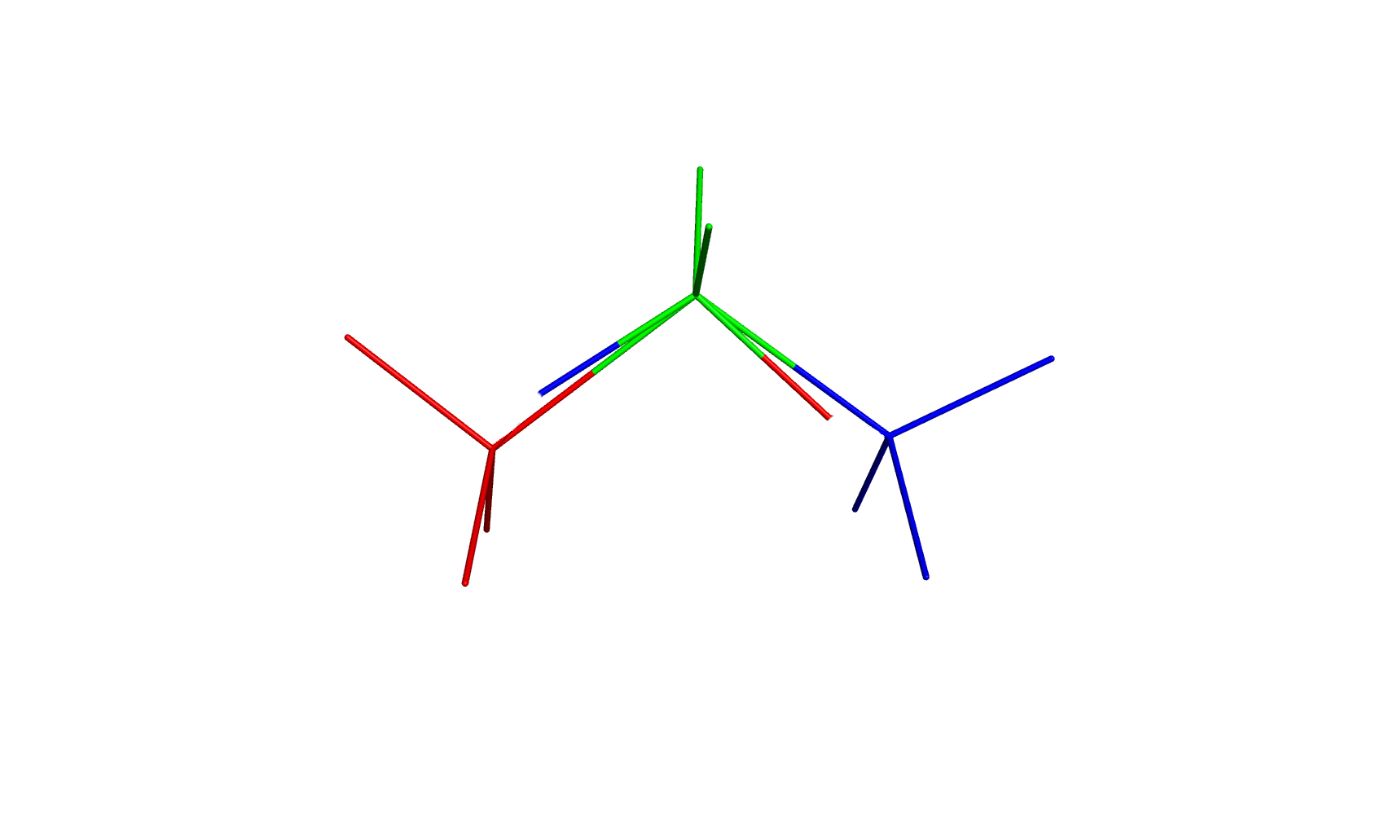
\includegraphics[width=0.5\textwidth]{img/imgfep1.png}
		\caption{Exemplifying \ac{FEP} calculations in \ac{CAST}}
		\label{fig:FEP1}
	\end{figure}
	The original Ethane is modified by adding another CH3-group + H to one of the ends of the molecule. In the next step the atoms belonging to both the starting and the final step have to be identified (they are marked in green in the figure). Those atoms don’t need to be modified in the input file and are always present in the simulation. The atoms marked in blue are the ones belonging to the starting system and are phased “out” during the simulation. All atoms belonging only to the starting point have to be marked with an \textit{IN} in the coordinate file after the bonding partner specification. The atoms belonging to the final state of the system have to be marked with an \textit{OUT} after the bonding partner specification. The modified file is shown in the following:\\~\\
	\begin{figure}[h]
		\centering
		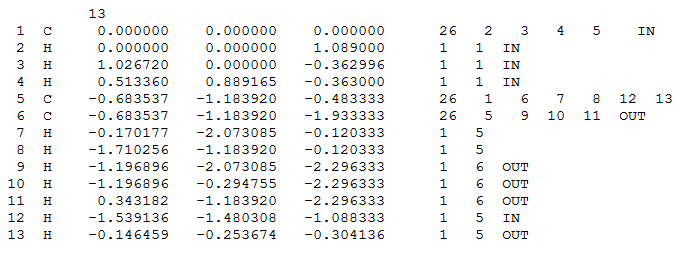
\includegraphics[width=0.95\textwidth]{img/imgfep2.png}
		\caption{Modifies tinker input style for \ac{FEP} calculations}
		\label{fig:FEP2}
	\end{figure}~\\
	One condition of the dual topology paradigm is that the atoms only belonging to the start point and end point must not interact with each other during the calculation. \ac{CAST} takes care of this automatically by excluding all angles, dihedrals or non-bonded interactions involving atom belonging to \textit{IN} or \textit{OUT}.
	\ac{FEP} calculations can be modified with various parameters.

	\begin{tabularx}{\textwidth}{l|X|X}
		variable & effect & default \\
		\hline
		\ifdevmode \textbf{FEPlambda} & Final value for order parameter. Doesn’t need to be changed at all & float [1.0] \\ \fi 
		\textbf{FEPdlambda} & Lambda increment. ${FEPdlambda}^{-1} =$ number of \ac{FEP} windows.	& float [0.05] \\
		\textbf{FEPvdwcouple} & Controls coupling of \ac{VdW} interactions (see XX) \ifdevmode \colorbox{red}{what is XX? see where?} \fi & float [1.0] \\
		\textbf{FEPeleccouple} & Controls coupling of electrostatics (see XX) \ifdevmode \colorbox{red}{what is XX? see where?} \fi
		& float [1.0] \\
		\textbf{FEPvshift} & Value for the \ac{VdW} shifting parameter in the softcore potential \ifdevmode \colorbox{red}{what even?} \fi & float [1.0] \\
		\textbf{FEPcshift} & Value for shifting parameter in the electrostatic potential & float [1.0] \\
		\textbf{FEPequil} & Number of equilibration steps in each window & integer [10] \\
		\textbf{FEPsteps} & Number of production steps in each window & integer [10]\\
		\textbf{FEPfreq} & Frequency of \ac{FEP} output & integer [1000] \\
	\end{tabularx}\\~\\

	\ac{FEP} calculations produce two output files: alchemical.txt and FEP_Results.txt. Alchemical contains detailed information about electrostatic and \ac{VdW} interactions for the current lambda value. Furthermore, the current temperature and free energy change is displayed. The file FEP_Results.txt contains the total free energy change for the simulation and for each window.
	The \ac{FEP} implementation is part of the \ac{MD} code. Thermostats, barostats boundary conditions and all other parameters needed can be controlled with the corresponding \ac{MD} variables.

	%%%% Dimer Method (DIMER) %%%%
	\subsection{DIMER - Dimer Method}
	The "dimer size" (magnitude of dimer vector) in the dimer method\supercite{dimermethod} can be controlled via "DIMERdistance" (default "0.01").
	It is possible to adjust the maximum rotational force during the dimer translation. The dimer translation is interrupted and the dimer is rotated into the minimum in case this limit is exceeded. The key controlling this value is called "DIMERtflimit" (default "0.01").
	The maximum number of iterations for the dimer rotation and translation steps can be set in the combined "DIMERmaxit" option, which takes two parameters where the first one limits the number of rotation iterations per translation step while the second one represents the maximum number of translations (default value: "20 100", maximum number of total dimer iterations is therefore ).
	The convergence criterion for the dimer rotation (the angle that needs to be undercut) in degrees can be adjusted using "DIMERrotconvergence" (default: "5.0").

	\begin{tabularx}{\textwidth}{l|X|X}
		variable & effect & default \\
		\hline
		\textbf{DIMERdistance} & Controls magnitude of dimer vector & float [0.01] \\
		\textbf{DIMERtflimit} & Controls magnitude of dimer force & float [0.01] \\
		\textbf{DIMERmaxit}& Controls rotation steps per translation and total translation steps & integer, integer [20 100]\\
		\textbf{DIMERrotconvergence} & Convergence criterium for rotation in degree & float [5.0] \\
	\end{tabularx}

	%%%% Global Optimization (GO) %%%%
	\subsection{GO - Global Optimization}
	The total number of steps for the global optimization routines is set by "Iterations" (default "1000"). \ac{CAST} will save all minima between E_0 (current lowest energy) and $E_0 + D$ where the value of D is adjusted with the "Erange" keyword (default "0.0").
	If the current step does not result in a newly accepted minimum, \ac{CAST} will select a new starting point. The key "GOfallback" selects either a simple fallback to local / global minimum (value "LAST_GLOBAL", default) or an evolutionary selection algorithm (value "EVOLUTION").

	\begin{tabularx}{\textwidth}{l|X|X}
		variable & effect & default \\
		\hline
		\textbf{Iterations} & Number of iterations & 1000 \\
		\textbf{Erange} & Energy range for output & 0.0 \\
		\textbf{GOfallback} & Type of fallback & LAST_GLOBAL \\
	\end{tabularx}

	%% Starting point selection
	\subsubsection{Starting point selection}
	\textbf{Simple Fallback} \\
	This method uses the parameter "GOfallback_limit" to determine how often the program can use a specific minimum as a starting point. If the limit for the last accepted minimum is reached, \ac{CAST} uses the current "global" minimum instead. If the limit for this minimum has also been reached, \ac{CAST} stops.\\~\\

	%% Evolutionary selection
	\textbf{Evolutionary selection} \\
	This algorithm selects a new starting point among a limited number of minima N. (The limit is set via "GOincluded_minima" and defaults to 10.)
	A roulette selection algorithm is applied where the fitness of the respective structures is de-termined based on their energetic rank. A lower L and an upper bound H for the fitness can be specified using "GOfitness_bounds" (default "0.5 1.0") where minimum N has fitness L and minimum 1 has fitness H.
	The interpolation between those points (1,H) -> (N,L) can be controlled by "GOfitness" where the value "LINEAR" (default) denotes linear interpolation while "EXPONENTIAL" activates exponential decay.
	\ac{CAST} makes up to 100 attempts to select a minimum which hasn’t reached the limit yet and stops if none is found.

	\begin{tabularx}{\textwidth}{l|X|X}
		variable & effect & default \\
		\hline
		\textbf{GOfallback_limit} & Number of times a minimum can be used & - \\
		\textbf{GOincluded_minima} & Number of minima to look for new starting point & 10 \\
		\textbf{GOfitness_bounds} (2 values) & Lower and upper bound for fitness & 0.5 1.0 \\
		\textbf{GOfitness} & Interpolation between \textbf{GOfitness_bounds} & LINEAR \\
	\end{tabularx}
	\\~\\

	%% Metropolis Criterion
	\textbf{Metropolix Criterion} \\
	The global optimization routines in \ac{CAST} evaluate the energy of a certain conformation (E) using the Metropolis criterion (MEC).
	\begin{equation}
	R < e^{-\frac{E-E_0}{kT}}
	\end{equation}
	\\~\\
	with R: Random number ($0 <= R <= 1$)
	and E: Evaluated energy
	and $E_0$: Reference energy
	and k: Boltzmann constant
	and T: Temperature\\~\\

	The reference energy E_0 can either be the energy representing the most stable structure (current "global minimum") or the last local minimum energy. The corresponding control option is called "GOmetrolocal" and defaults to 0 (off) which means that the current global minimum energy is used in the conditional. A value of "1" will make \ac{CAST} use the "current local minimum" energy (the starting point of the current iteration). If the MEC is not met, the conformation will be discarded.
	The temperature used is controlled via "Temperature" and defaults to "298.15". It is multiplied by a factor, adjusted via "Tempscale" (default: "1.0").\\~\\

	\begin{tabularx}{\textwidth}{l|X|X}
		variable & effect & default\\
		\hline
		\textbf{GOmetrolocal} & Use global or current local minimum energy as reference; 0 = no, yes = 1 & 0 \\
		\textbf{Temperature} & Temperature in Kelvin & 298.15 \\
		\textbf{Tempscale} & Multiplication factor for temperature & 1.0
	\end{tabularx}

	%% Monte Carlo
	\subsubsection{Monte Carlo (MC(M))}
	The MC(M) simulation will move randomly across the PES and evaluate the reached point either directly or after local optimization. The "MCminimization" option turns minimization on (value "1"; default) or off (value "0"). \\~\\
	\textbf{Move types}\\~\\
	\ac{CAST} can move to the next sampling point during MC in three different ways, controlled via the "MCmovetype" option (default "1"). A value of "2" will make the program carry out the contortion in Cartesian space (where the "MCstep_size" option with a default value of "2.0" will restrict the absolute value of the distortion vector). The value "1" represents direct rota-tion of randomly selected main dihedral angles (see 1.5). A value of "0" means that the tar-get conformation is not obtained directly by adjusting dihedrals but the conformational change will be achieved by applying quadratic bias potentials on the main dihedrals towards the target conformation during a local optimization process ("MCmax_dihedral" restricts the maximum distortion of a dihedral angle; default "160.0"). \\

	\begin{tabularx}{\textwidth}{l|X|X}
		MCmovetype value & Move type & Associated options \\
		\hline
		0 & Biased main dihedral optimization & MCmax_dihedral \\
		1 & Main dihedral & MCmax_dihedral \\
		2 & Cartesian & MCstep_size \\
	\end{tabularx}
	\\~\\
	The number of distorted dihedrals is selected randomly in case of a "MCmovetype" value of 0 or 1 (biased or direct main dihedral adjustment).
	\begin{equation}
	N = - log (R) + 1
	\end{equation}
	with R being a random number between 0 and 1 and N being the number of distorted rotated dihedrals.\\~\\
	\begin{tabularx}{\textwidth}{l|X|X}
		variable & effect & default \\
		\hline
		MCminimization & Turn minimization on or off; 0 = off, 1 = on & 1 \\
		MCmovetype & Movetype to go to next sampling point & 1 \\
		MCstep_size & Absolute value of distortion vector & 2.0 \\
		MCmax_dihedral & Maximum distortion of dihedral angle in degre & 160.0 \\
	\end{tabularx}
	\\~\\

	%% Tabu Search
	\subsubsection{Tabu Search (TS)}
	The \acf{TS} process in \ac{CAST} is essentially an alternating combination of the dimer method\supercite{dimermethod}and the local optimization process.
	If a certain number of \ac{TS} iterations does not yield a new, accepted minimum the diversification search process (DS; MCM is used here) is executed. The option controlling how many steps need to fail before DS comes into place is called "TSdivers_threshold" (default "25").
	The "TSdivers_iter" option (default "30") represents the number of iterations in the diversifi-cation routine.
	If you want \ac{CAST} to start with DS iterations instead of \ac{TS} iterations you can set "TSmc_first" to "1" (default "0").\\~\\

	\begin{tabularx}{\textwidth}{l|X|X}
		variable & effect & default \\
		\hline
		TSdivers_threshold & Number of failed steps before diversification search & 25 \\
		TSdivers_iter & Number of iterations during diversification & 30 \\
		TSmc_first & Start with diversification instead of Tabu Search iterations; 0 = no, 1 = yes & 1 \\
	\end{tabularx}
	\\~\\

	%% Output
	\subsubsection{Output}
	The output (verbosity > 1) includes 15 columns (with NA being the number of currently accepted minima):\\
	\begin{itemize}
		\item Method (MC, MCM or TS)
		\item Current iteration
		\item \textbackslash \ifdevmode \colorbox{red}{I guess that means blank line, does it?} \fi
		\item Maximum number of iteration
		\item Index of current minimum in the interval (0, NA)
		\item Current minimum energy (starting point of current step)
		\item "Transition step" energy (energy after distortion / dimer method without optimization)
		\item New minimum energy (after optimizing the "transition step" structure).
		\item Identifier for acceptance (A = accepted; R = rejected)
		\item Acceptance information
		\begin{itemize}
			\item ok = new minimum, but not lowest
			\item GM = new minimum, lowest
			\item energy = rejected because of metropolis criterion
			\item broken = Configurational feature of the structure broken
			\item tabu = already visited minimum
		\end{itemize}
		\item Number of accepted minima (NA)
		\item Number of minima within the energy range (see 5.5.3 \ifdevmode \colorbox{red}{This number needs to be updated} \fi)
		\item Current temperature used for the metropolis criterion (see 5.5.5 \ifdevmode \colorbox{red}{This number needs to be updated} \fi)
		\item Iteration Runtime
		\item Number of CPU clock ticks required for current iteration
	\end{itemize}

	Example:\\
	\begin{lstlisting}
	MCM; 87/100; 0 -2.0604e+02; -1.8566e+02; -2.0516e02;
	R (energy) 1 1 (47.04 K, 3.37s (33701 ticks))
	\end{lstlisting}~\\

	%%%% Trajectory alignment (ALIGN) %%%%
	\subsection{ALIGN - Trajectory Alignment}
	 The trajectory alignment task allows the alignment of molecular dynamics output structures via Kabsch alignment. Alignment is performed for translational and rotational motion. THe trajectory alignment also allows to calculate several RMSD values. The standard RMSD, the dRMSD and the Holm and Sander distance. If no alignment is performed beforehand the RMSD is calculated among the unaligned snapshots. CAST provides the following optionsfor the task ALIGN: \\~\\

	\begin{tabularx}{\textwidth}{l|X|X}
		variable & effect & default\\
		\hline
		traj_align_bool & Switch alignment on or off, false = off, true = on & true\\

	\end{tabularx}
	\ifdevmode
	\colorbox{red}{HERE IS STILL WORK TO BE DONE}
	\fi

	%%%% Entropy calculations (ENTROPY) %%%%
	\subsection{ENTROPY - Trajectory Alignment}
	For further analysis of MD output CAST provides the calculation of entropy contributions. The entropy calculation is based on the quasi-harmonic approximation by Karplus and further extended versions of this approximation by Knapp and Schlitter. Calculations can be per-formed in cartesian or internal coordinates for all or only several snapshots. The following options are provided by CAST: \\~\\

	\begin{tabularx}{\textwidth}{l|X|X}
		variable & effect & default\\
		\hline
		entropy_alignment & Switch alignment on or off, false = off, true = on & true\\

	\end{tabularx}
	\ifdevmode
	\colorbox{red}{HERE IS STILL WORK TO BE DONE}
	\fi

	%%%% Principal Component Analysis (PCA) %%%%
	\subsection{PCA - Principal Component Analysis}
	The PCA task performs a principal component analysis on MD trajectories produced by CAST. Several output files can be generated, next to the standard output of the produced new coordinates. \\~\\

	\begin{tabularx}{\textwidth}{l|X|X}
		variable & effect & default  \\
		\hline
		pca_alignment & Switch alignment on or off, false = off, true = on & true\\

	\end{tabularx}
	\ifdevmode
	\colorbox{red}{HERE IS STILL WORK TO BE DONE}
	\fi

	%%%% Boundry Conditions %%%%
	\subsection{Boundary Conditions}

	\ifdevmode \colorbox{red}{We should put this section somewhere else, not as a subsection of TASKS...} \fi

	CAST features two types of boundary conditions: spherical and periodic. Spherical boundary conditions can be applied with an energy interface if desired, periodic boundaries are limited to the force field interfaces.

	%% Spherical boundaries
	\subsubsection{Spherical boundaries}
	Spherical boundaries apply a harmonic potential on particles which drift farer away from the geometric center of the simulation than a certain threshold. There are 7 input parameters in total which are defined in a single line in the input file. \\~\\

	\begin{tabularx}{\textwidth}{l|X|X|X|X|X|X|X}
		keyword & param1 & param3 & param4 & param5 & param6 & param7 \\
		\hline
		MDspherical & active & Radius1 & Radius1 & Force1 & Force2 & Exp1 & Exp2 \\
		MDspherical & 1 & 30.0 & 0.0 & 10.0 & 0.0 & 2 & 0 \\
	\end{tabularx}~\\

	Effects of the input variables in detail:\\~\\
	\begin{tabularx}{\textwidth}{l|X|X}
		\textbf{variable} & effect & default \\
		\hline
		\textbf{Active} & Switches spherical boundaries on or off; 0 = off, 1 = on & 0 \\
		\textbf{Radius1} & Distance for the first potential in Å & none \\
		\textbf{Radius2} & Distance for the second potential in Å & none \\
		\textbf{Force1} & Force constant for inner radius & none \\
		\textbf{Force2} & Force constant for outer radius & none \\
		\textbf{Exp1} & Exponent for inner potential & None, only 2 and 4 are reasonable \\
		\textbf{Exp2} & Exponent for outer potential & None, only 2 and 4 are reasonable \\
	\end{tabularx}~\\
	There are two potentials that can be applied: a standard harmonic potential if only the vari-ables with index 1 are used and if the variables with index 2 are also used, a second harmon-ic potential with a different radius can be applied.
	Force constants are given in $\frac{kcal}{mol}$. Negative force constants push atoms away from the center, positive force constants push it toward the center.

	\subsubsection{Periodic boundary conditions}
	Periodic boundary conditions can be used to simulate periodic systems. The basic idea is to choose the smallest possible unit cell in the systems as the simulated system and virtually copy it indefinitely in all directions to generate an infinite system. In the actual simulation only the conditions of the initial unit cell are calculated. The infinity is generated by the fact, that particles that leave the simulation box reenter from the opposite side. PBC are usually used for the simulation of solvated macromolecules or other mixtures, as well as bulk gases, liquids and crystals. Crucial parameters for the correct behavior of the boundary conditions are the size and shape of the unit cell as well as the chosen cutoff radius. Periodic bounda-ries are enabled in a single line in the input file with the keyword Periodics.\\
	\begin{tabularx}{\textwidth}{l|X|X|X|X}
		\textbf{keyword} & param1 & param2 & param3 & param4 \\
		\hline
		\textbf{periodics} & active & x-dim & y-dim & z-dim \\
		\textbf{periodics} & 1 & 10.0 & 10.0 & 10.0 \\
	\end{tabularx}\\~\\~\\
	Effects of the input variables in detail:\\~\\
	\begin{tabularx}{\textwidth}{l|X|X}
		\textbf{variable} & effect & default \\
		\hline
		\textbf{active} & Switch periodics on or off, 0 = off, 1 = on & 0 \\
		\textbf{x-dim} & Box-dimension in x-direction in Å & 0 \\
		\textbf{y-dim} & Box-dimension in y-direction in Å & 0 \\
		\textbf{z-dim} & Box-dimension in z-direction in Å & 0 \\
	\end{tabularx}~\\


	%%%%%%%%%%%%%%%%%%%%%%%%%%%%%%%%%%%%
	%%%%                            %%%%
	%%%% CODING THE CAST FRAMEWORK  %%%%
	%%%%                            %%%%
	%%%%%%%%%%%%%%%%%%%%%%%%%%%%%%%%%%%%
	\ifdevelopment
	\newpage
	\section{Coding within the CAST Framework}
	Lorem Ipsum here be text it the future \\
	\ifdevmode \colorbox{red}{Once CAST4 is up and running we should pt some information on the code here.} \fi
	\fi


	%%%%%%%%%%%%%%%%%%%%%%%%%%%%%%%%%%%%
	%%%%                            %%%%
	%%%% IF SOMETHING GOES WRONG    %%%%
	%%%%                            %%%%
	%%%%%%%%%%%%%%%%%%%%%%%%%%%%%%%%%%%%
	\newpage
	\section{What to do if something goes wrong}
	If you encounter unexpected behavior when using \ac{CAST}, you may contact the developers for support. In order to properly categorize the issue you may be encountering, consider running \ac{CAST} again with \textit{verbosity} set to a very high number (for example \textit{500}, or, if this produces too much data, \textit{20}) and sending us the text-output as well as the generated files. \\

	Even though the \ac{CAST} source code is currently not available to the public, we provide a dedicated \textit{github} repository for providing feedback to users and resolve issues. It may be found at \url{https://github.com/djmuw/cast_feedback}. If you do not want to use the \textit{github} repository, you can also write us an E-Mail.

	%%%%%%%%%%%%%%%%%%%%%%%%%%%%%%%%%%%%
	%%%%                            %%%%
	%%%%      HOW TO CITE CAST      %%%%
	%%%%                            %%%%
	%%%%%%%%%%%%%%%%%%%%%%%%%%%%%%%%%%%%
	\newpage
	\section{How to cite CAST}

	%%%%%%%%%%%%%%%%%%%%%%%%%%%%%%%%%%%%
	%%%%                            %%%%
	%%%%  CONTACT AND SUPPORT       %%%%
	%%%%                            %%%%
	%%%%%%%%%%%%%%%%%%%%%%%%%%%%%%%%%%%%
	\newpage
	\section{Contact and Support}
	\href{mailto:cast@chemie.uni-wuerzburg.de}{cast@chemie.uni-wuerzburg.de} \ifdevmode \colorbox{red}{we should really acquire this mail adress, better than not having it.} \fi \\~\\

	Working Group Prof. Dr. Bernd Engels\\
	Institute for Physical and Theoretical Chemistry\\
	Julius-Maximilians University Wuerzburg\\
	Emil-Fischer-Strasse 42\\
	97074 Wuerzburg\\
	GERMANY\\~\\
	Technical Support via:\\
	\url{https://github.com/djmuw/cast_feedback}\\
	or\\
	\href{mailto:cast@chemie.uni-wuerzburg.de}{cast@chemie.uni-wuerzburg.de}\\

	%%%%%%%%%%%%%%%%%%%%%%%%%%%%%%%%%%%%
	%%%%                            %%%%
	%%%%  BIBLIOGRAPHY              %%%%
	%%%%                            %%%%
	%%%%%%%%%%%%%%%%%%%%%%%%%%%%%%%%%%%%
	\newpage
	\section{Bibliography}
	\printbibliography



\end{document}
